% Roles of the six blocks in each fold (F2 of the review). Fold 0 is the development fold of FSDD
% and EEGMMIDB; fold 1 tests on the block that fold 0 validated on, so both leave the headline.
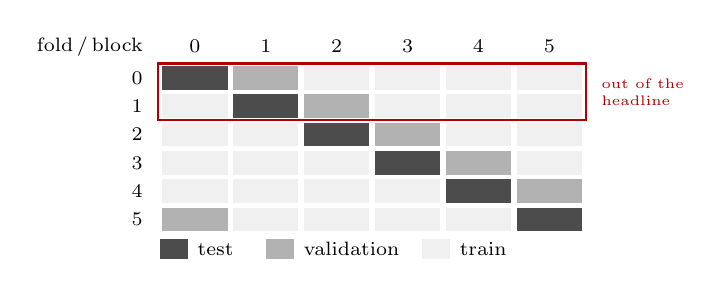
\begin{tikzpicture}[font=\scriptsize, x=9mm, y=3.6mm]
  \foreach \b in {0,...,5} \node at (\b+0.5,0.6) {\b};
  \node[anchor=east] at (-0.1,0.6) {fold\,/\,block};
  \foreach \f in {0,...,5} {
    \node[anchor=east] at (-0.1,-\f-0.5) {\f};
    \pgfmathtruncatemacro{\v}{mod(\f+1,6)}
    \foreach \b in {0,...,5} {
      \ifnum\b=\f \def\cell{black!70}\else\ifnum\b=\v \def\cell{black!30}\else\def\cell{black!6}\fi\fi
      \fill[\cell] (\b+0.04,-\f-0.92) rectangle (\b+0.96,-\f-0.08);
    }
  }
  \draw[red!70!black, thick] (-0.02,0) rectangle (6.02,-2);
  \node[red!70!black, anchor=west, align=left, font=\tiny] at (6.1,-1) {out of the\\headline};
  \fill[black!70] (0,-6.9) rectangle (0.4,-6.2); \node[anchor=west] at (0.4,-6.55) {test};
  \fill[black!30] (1.5,-6.9) rectangle (1.9,-6.2); \node[anchor=west] at (1.9,-6.55) {validation};
  \fill[black!6] (3.7,-6.9) rectangle (4.1,-6.2); \node[anchor=west] at (4.1,-6.55) {train};
\end{tikzpicture}
